\chapter[Arquitetura de Integração]{Arquitetura de Integração}

O diagrama da arquitetura de integração contém aspectos da solução de estrutura, energia, eletrônica e software. Assim, a visão geral dos subsistemas integrados que compões o projeto \textit{PillWatcher} está representada na Fig. \ref{fig:arq_integracao}, a qual ilustra os módulos conectados ente si para que o dispositivo funcione corretamente. 

Dessa forma, a estrutura do dispositivo tem o cuidado de acoplar os componentes eletrônicos necessários na parte interna, como as placas de circuito impresso (PCI), os sensores e os \textit{drivers}. 

Para a alimentação dos componentes no dispositivo a solução de energia projetou uma fonte de 12 V e 15 A para realizar a alimentação dos dispositivos elétricos e eletrônicos do sistema. Os componentes eletrônicos exigem uma tensão inferior à disponibilizada pela fonte, dessa forma, será utilizado um regulador de tensão de 12 V para uma saída de 5 V e 8 A, representado no diagrama \ref{fig:integracao_eletrônica_energia} como a fonte de 5 V e 8 A.

A solução eletrônica está representada pelos subsistemas do modulo de medição, módulo de interação e módulo de acionamento dos atuadores. A conexão entre esse módulos é feita pela central de controle representada pelo sistema embarcado (Computador de Placa Única e microcontroladores). Para comunicação entre a solução eletrônica e o \textit{backend} da arquitetura de software, representado pelos módulos de exposição, serviços negociais, armazenamento de dados e fila, é utilizado os protocolos de comunicação MQTT e HTTP. O \textit{front-end} é representado pelo módulo de interação e se comunica com o \textit{back-end}, em específico o módulo de exposição, por meio do protocolo HTTP.

Cada integração dos subsistemas estão detalhadas nas seções seguintes deste capítulo. A seção \ref{pos_compontes} contém a descrição do posicionamento dos componentes eletrônicos. A seção \ref{alimentacao_componentes} expõe a fiação entre o submódulo do sistema de alimentação e os componentes eletrônicos. A seção \ref{app_dispositivo} apresenta os detalhes da interface com o usuário por meio do aplicativo, requisitos, procedimentos para a execução e comunicação do módulo do aplicativo com a central de controle.

\begin{landscape}
\begin{figure}[!htb]
    \centering
    \vspace{1cm}
    \hspace{-2cm}
    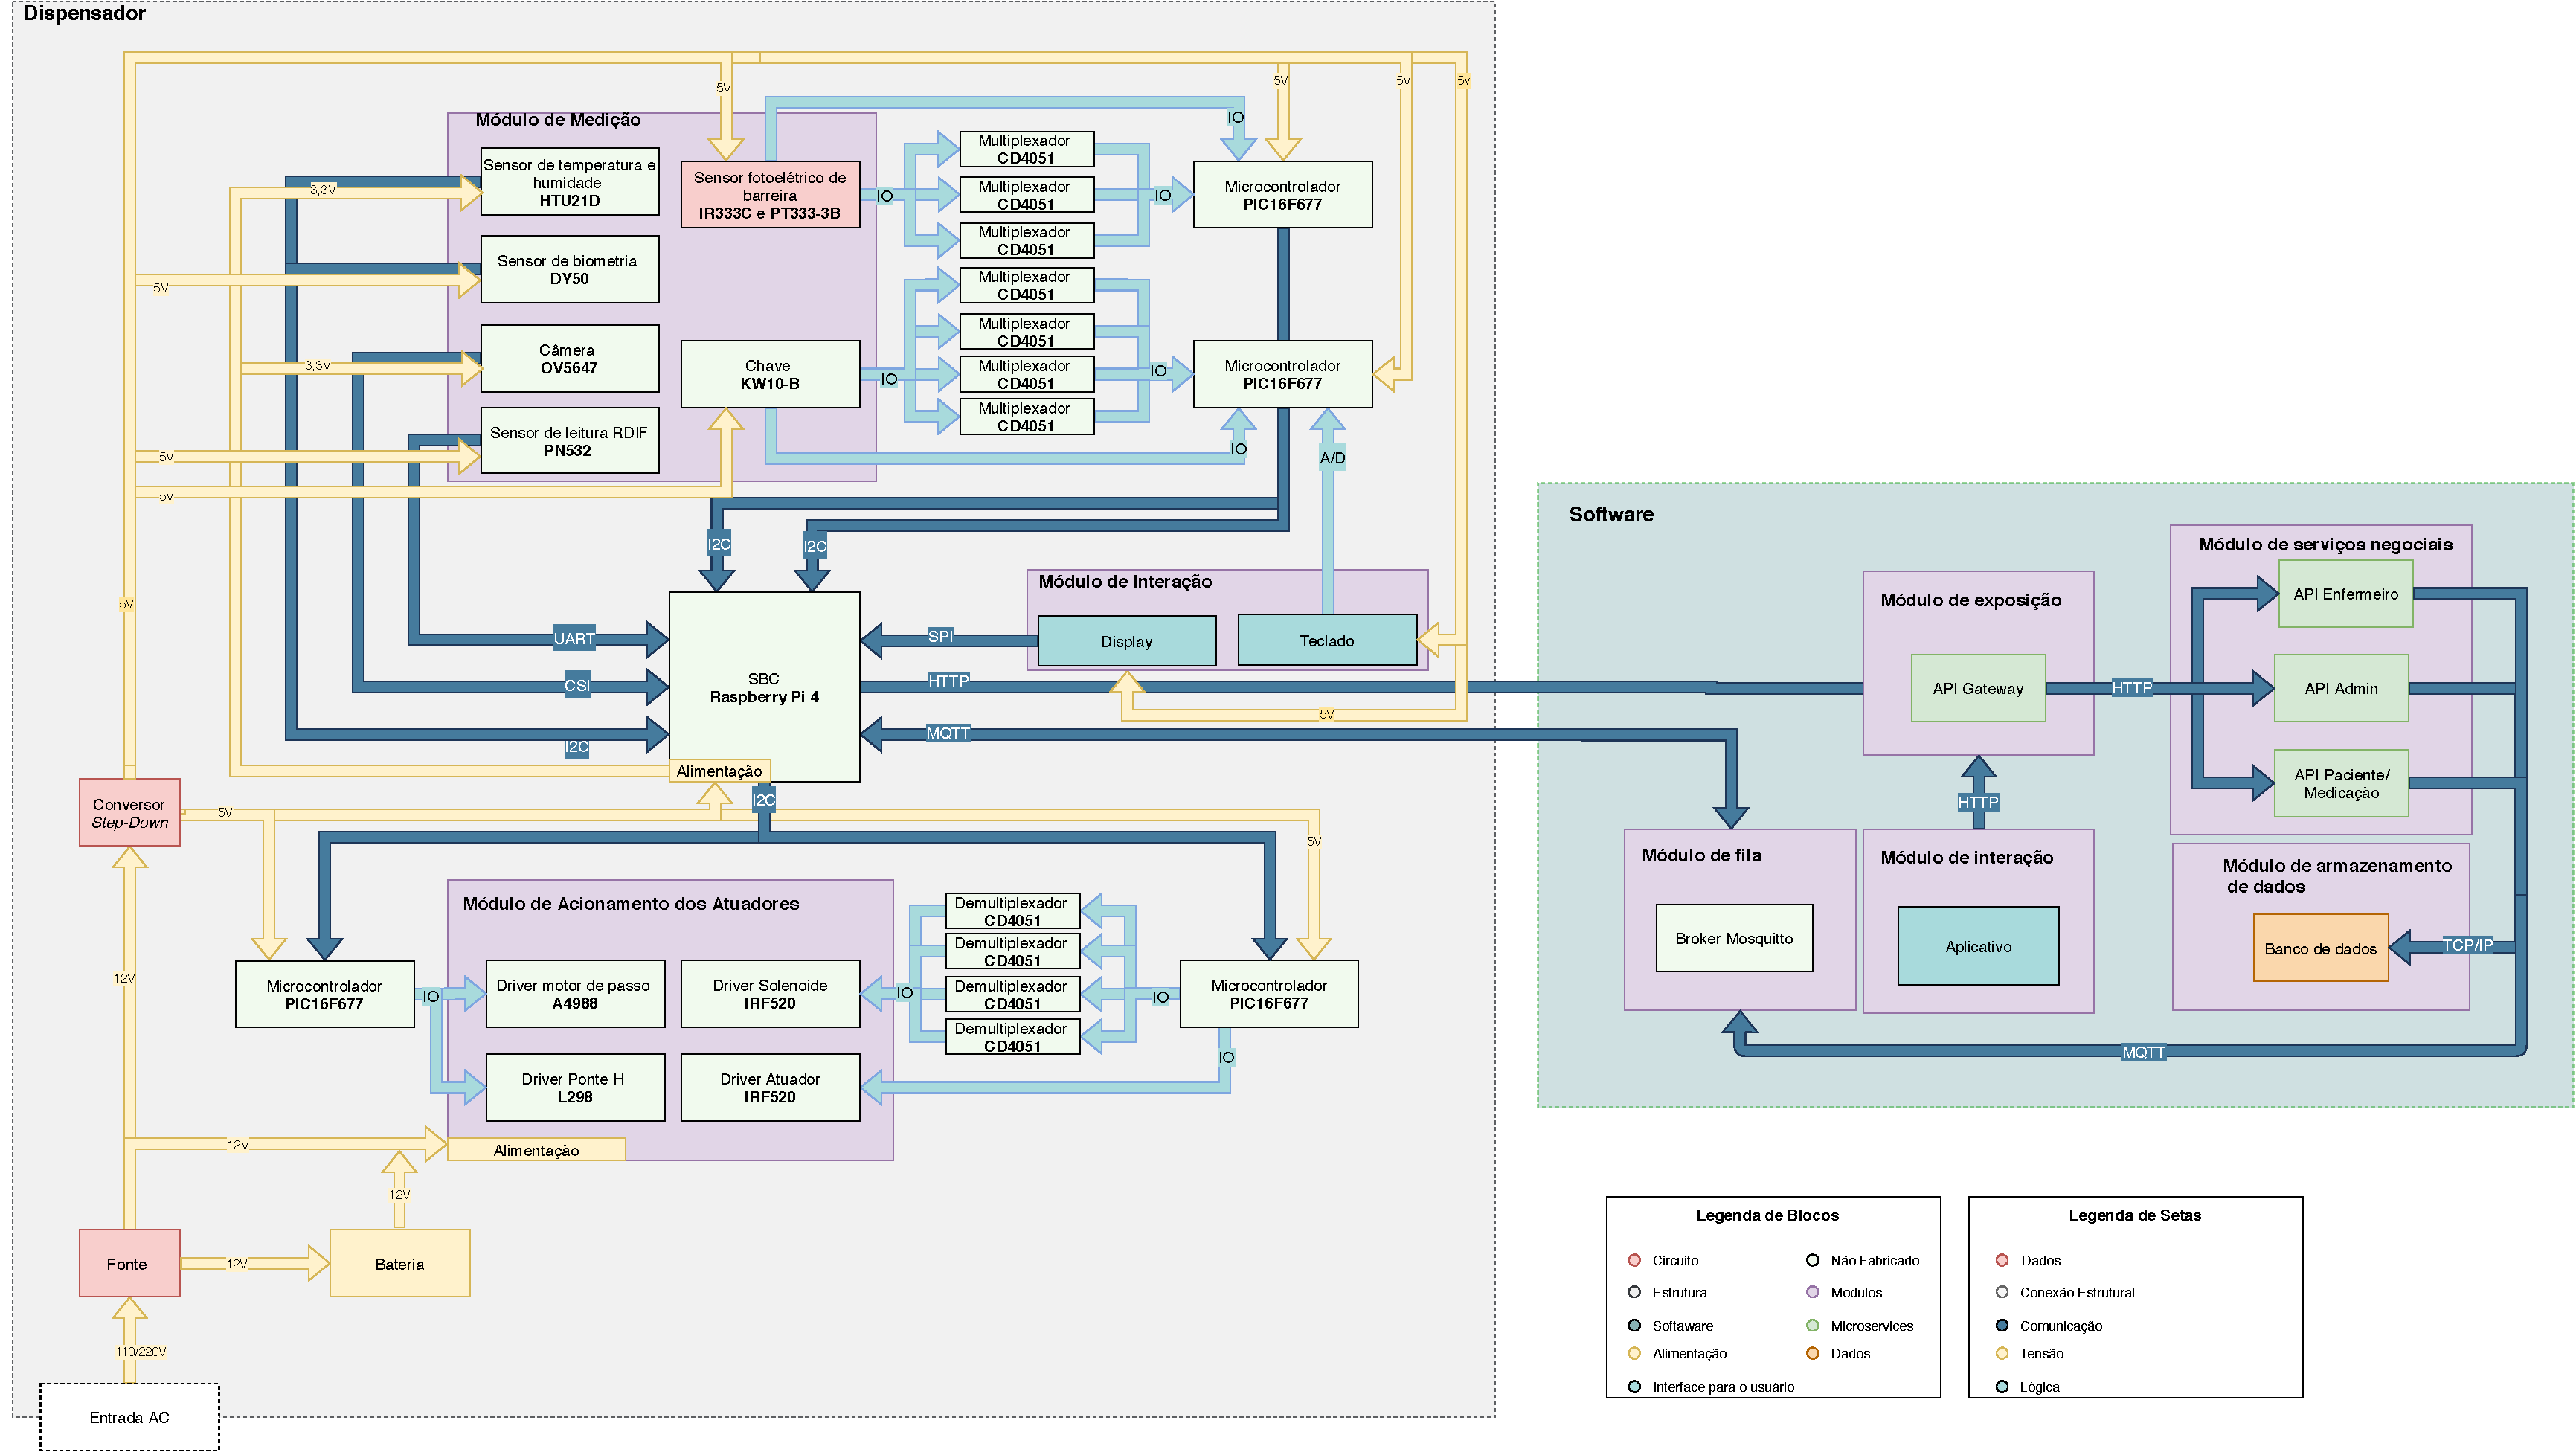
\includegraphics[width=1.5\textwidth, height=2\textheight,keepaspectratio]{figuras/integracao/integracao_geral.pdf}
    \vspace{-5pt}
    \caption{Diagrama de Integração de Subsistemas}
    \label{fig:arq_integracao}
\end{figure}
\end{landscape}


\section{Posicionamento dos Componentes dos Sistemas Elétricos e Eletrônicos}
\label{pos_compontes}

O posicionamento dos componentes foi escolhido em conjunto com as frentes de Eletrônica e Energia, baseado nas necessidades e limitações presentes nos sistemas físicos e arranjos disponíveis dentro da máquina. Os maiores pontos de decisões foram a facilidade de adaptação do usuário com o dispositivo e o melhor aproveitamento do espaço interno.

\subparagraph*{$\bullet$ Disposição do Sistema de Alimentação, Equipamentos Eletrônicos e Sistema Eletromecânico} \hfill

O posicionamento dos componentes do sistema de alimentação e equipamentos eletrônicos se deu pela facilidade de visualização do usuário, limites físicos associados a cabos e espaçamento disponível na estrutura.  

A disposição dos componentes externos é ilustrada na Fig. \ref{fig:Vista_componentes_externos}, podemos destacar a presença do visor, teclado e sensor de biometria no painel frontal da máquina. Além do mais, as mini-travas elétricas foram posicionadas nas portas do compartimento superior do dispositivo e na porta frontal.

\begin{figure}[H]
        \centering
        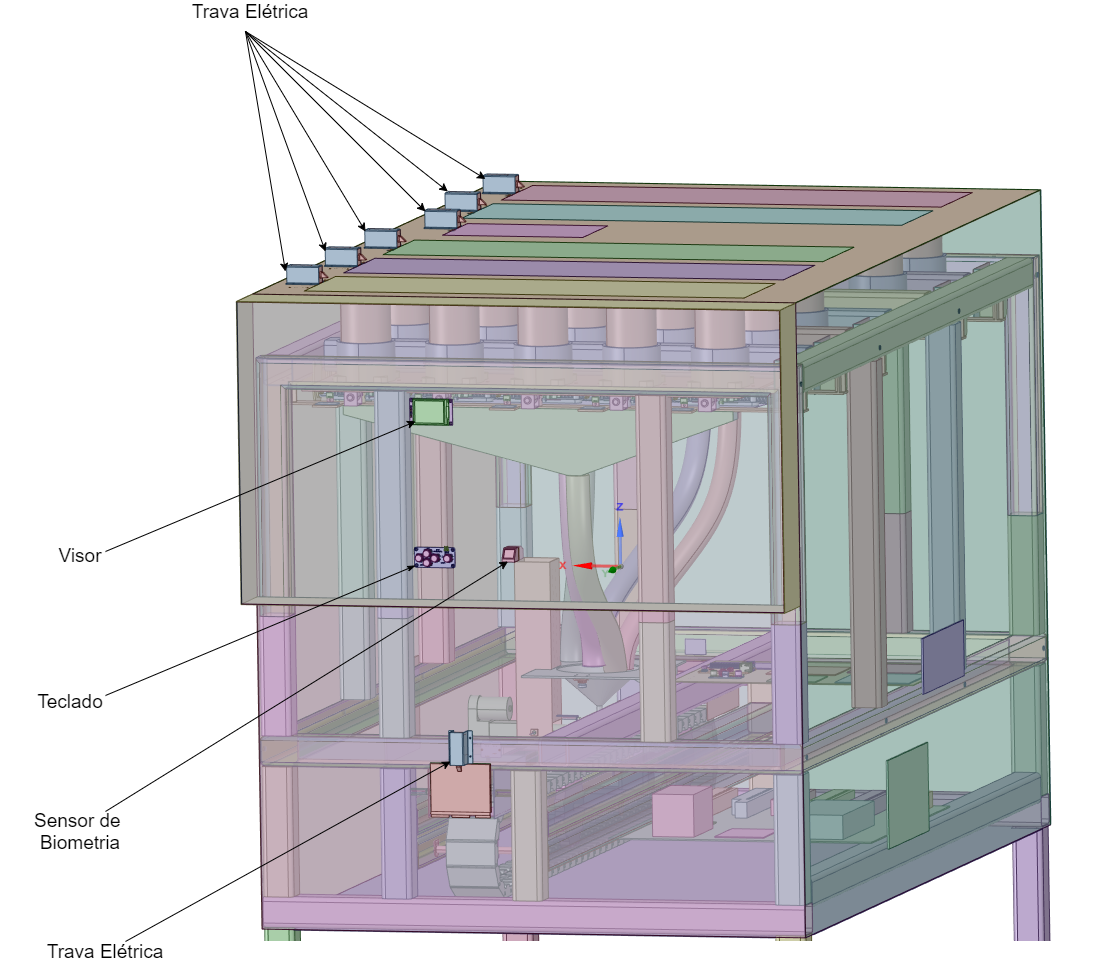
\includegraphics[width=0.70\textwidth]{figuras/integracao/Integracao_1.png}
        \caption{Posicionamento dos Componentes Eletrônicos Externos}
        \label{fig:Vista_componentes_externos}
    \end{figure}

Ao lado esquerdo do painel frontal, tem-se o local indicado para o posicionamento da bateria e fonte do sistema, sendo de fácil manutenção pela presença do componente removível posicionado logo à frente do atuador linear. Vale ressaltar como última observação que foi adaptado uma entrada na lateral para posicionamento dos copos.


 A partir da Fig. \ref{fig:Vista_componentes_porta}, a qual proporciona a visualização da porta de saída frontal do dispositivo é possível visualizar a distribuição de um par de  sensores fotoelétricos com sua respectiva Placa de Circuito Impresso (PCI) para verificar a retirada do copo com medicamento pelo enfermeiro, chave, fechadura eletrônica e \textit{Driver} do solenoide (\textbf{IRF520N}). Igualmente tem-se o posicionamento dos componentes eletrônicos na porta de saída traseira do dispositivo, a única diferença é que a porta traseira não possui trava eletrônica e o \textit{Driver} do solenoide.
 

\begin{figure}[H]
        \centering
        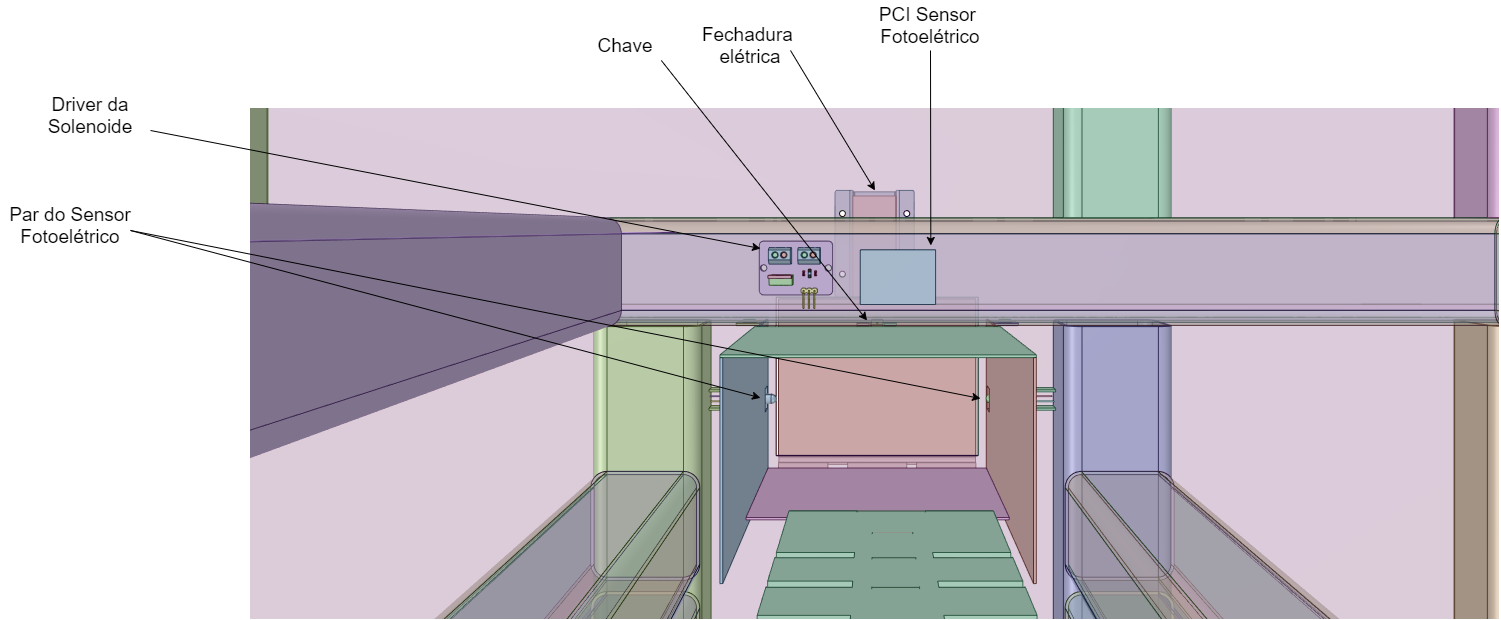
\includegraphics[width=\textwidth]{figuras/integracao/Integracao_2.png}
        \caption{Posicionamento dos componentes Eletrônicos na Porta Frontal}
        \label{fig:Vista_componentes_porta}
    \end{figure}
    
 Por meio da Fig. \ref{fig:integracao_3} observa-se que a \textit{Raspberry} se encontra posicionada próxima
 ao \textit{Step-down} e as PCIs da central de controle, dos módulos de medição e acionamento dos atuadores, as quais são descritas no Manual de Montagem e no plano de construção de eletrônica na seção \ref{sec:plano_de_construção}. Além no mais a \textit{Raspberry} necessita ficar a uma distância de até 300 mm da câmera, uma vez que tem a limitação do cabo \textit{flat}. 
 
 Logo abaixo das PCIS tem-se o local indicado para o posicionamento da bateria, a fonte do sistema, a PCI de carregamento e intertravamento da bateria, o \textit{Step-up} e os blocos de terminais de fios, sendo de fácil manutenção pela presença do componente removível posicionado logo à frente do atuador linear. Logo, o atuador linear  está próximo ao \textit{driver} (\textbf{IRF520N}) e a PCI do sensor de barreira que fica internamente ao reservatório de copos. 
    \begin{figure}[H]
        \centering
        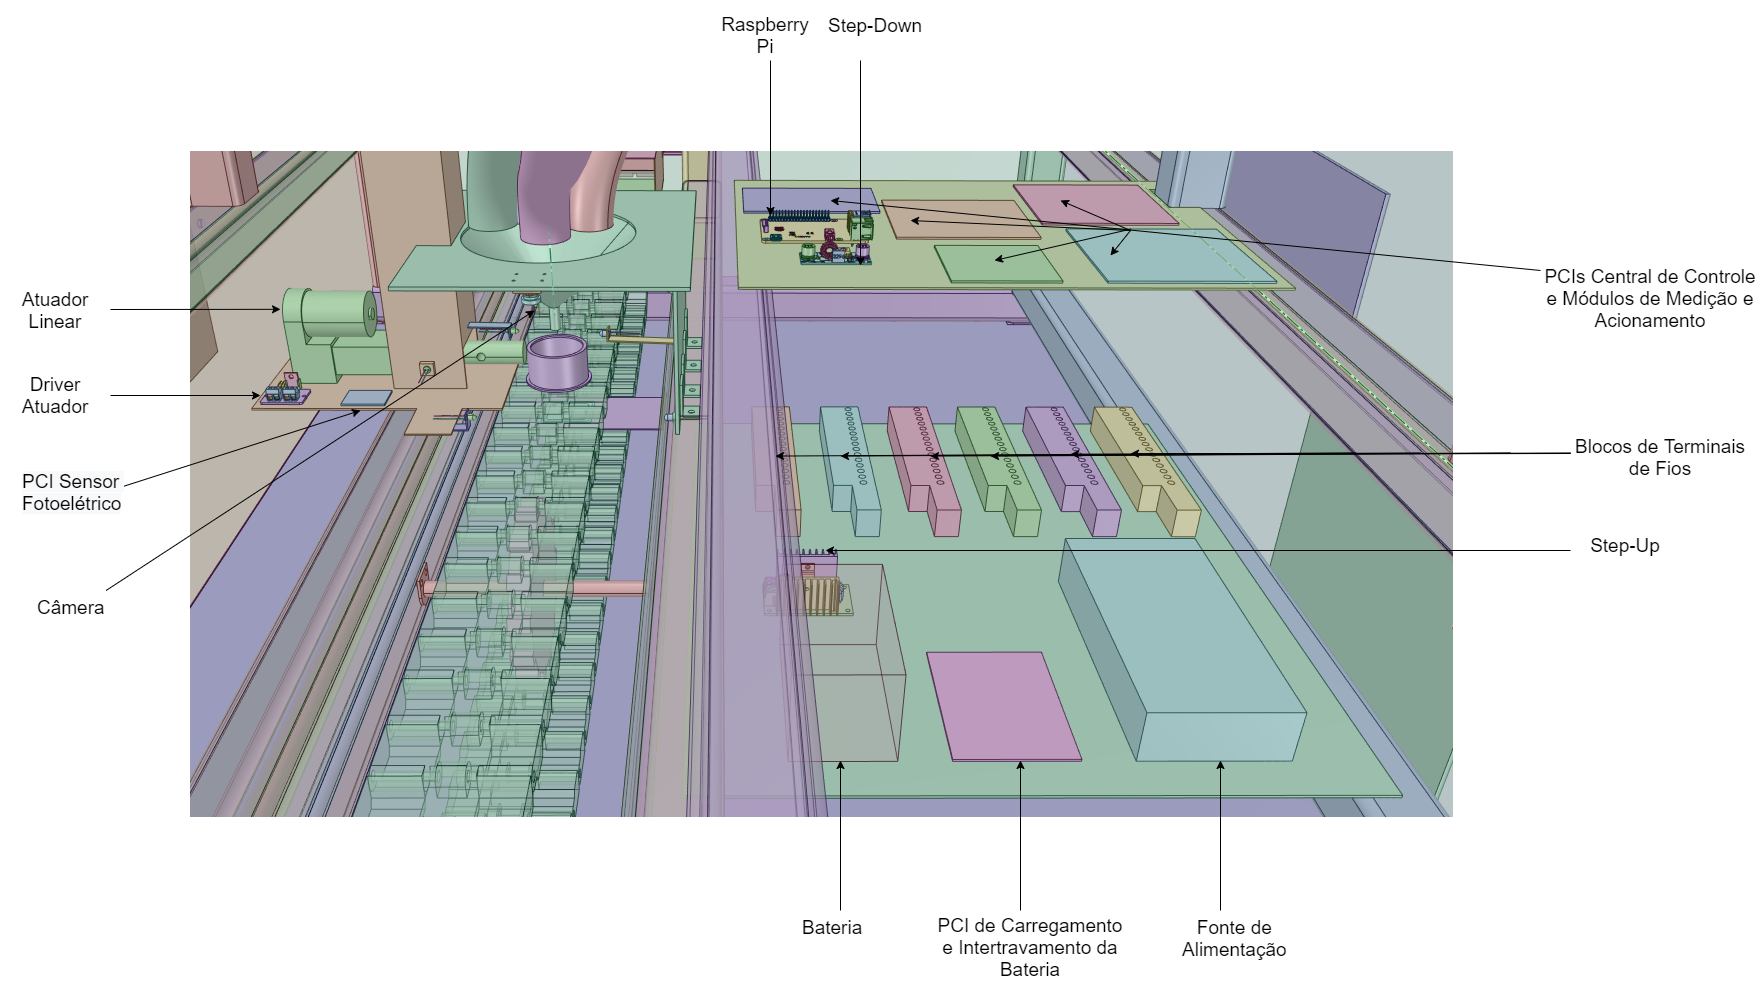
\includegraphics[width=\textwidth]{figuras/integracao/Integracao_3.png} 
        \caption{Disposição interna dos componentes Eletro-eletrônicos}
        \label{fig:integracao_3}
    \end{figure}
    
     %espaço para preencher a pagina
    \hspace{5cm}
    
    A Fig. \ref{fig:integracao_5} demonstra o posicionamento de três pares de sensor fotoelétricos com suas respectivas PCIs. Um dos sensores fotoelétricos está posicionado na altura da saída do funil, para verificação da queda dos comprimidos no copo, o outro dentro do reservatório de copos para averiguar se existem copos no reservatório e o último está localizado logo abaixo da câmera para detectar a passagem do copo e realizar o processamento de imagem. 
    
    %espaço para preencher a pagina
    \hspace{5cm}
    
    Além do mais, nessa ilustração é possível identificar o sensor de leitura RFID, o qual possui uma estrutura para sua sustentação, a qual necessariamente deve ficar até 50 mm da base do copo na esteira, uma vez que, a etiqueta RFID fixada na base do copo possui essa restrição.  
    
    \begin{figure}[H]
        \centering
        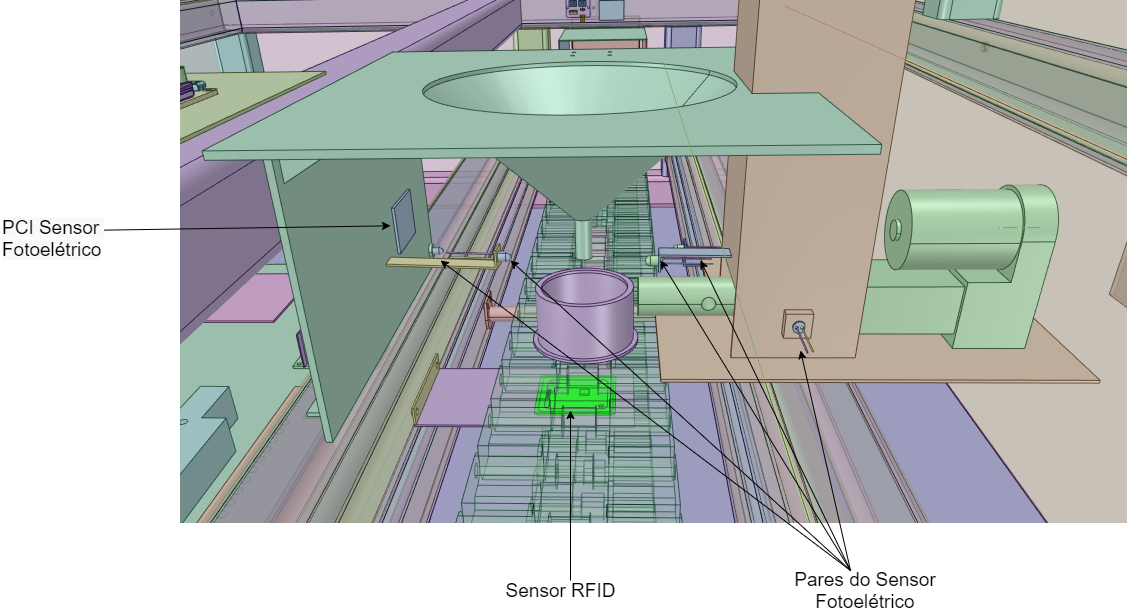
\includegraphics[width=1\textwidth]{figuras/integracao/integracao_5.png} 
        \caption{Disposição espacial do sistema de identificação do copo}
        \label{fig:integracao_5}
    \end{figure}
    
    
    O posicionamento dos solenoides e dos seus respectivos \textit{drivers} está explicitado na Fig. \ref{fig:integracao_4}, onde cada solenoide apresenta fixação de sua face superior na região inferior das mesas de apoio dos contêineres, enquanto seu braço de atuação está em coincidência com a comporta de cada contêiner. Para facilitar a visualização foi indicado apenas um solenoide e um \textit{driver} (\textbf{IRF520N}), mas cada contêiner possui esses componentes. 
    
    Outrossim, nessa Fig. é possível identificar a disposição das chaves para cada contêiner, as chaves e \textit{drivers} do solenoide (\textbf{IRF520N}) das cinco portas do compartimento superior.
     
    Os sensores fotoelétricos possuem diversos posicionamentos, uma vez que estes tem a função de verificar a queda de medicamentos e detectar o copo tanto reservatório, quanto na esteira. Dessa forma esse sensores são fixados conforme a \ref{fig:integracao_4} na letra A. Assim, para facilitar a visualização foi indicado apenas um par de sensores fotoelétricos que ficam posicionados na comporta, mas cada contêiner possui um par desses sensores. 
    
    Por último, cada mesa com cinco contêineres possui um motor de passo com seu respectivo \textit{driver} (\textbf{A4988}) conforme ilustrado na Fig. \ref{fig:integracao_4} na letra B.
    
    \begin{figure}[H]
        \centering
        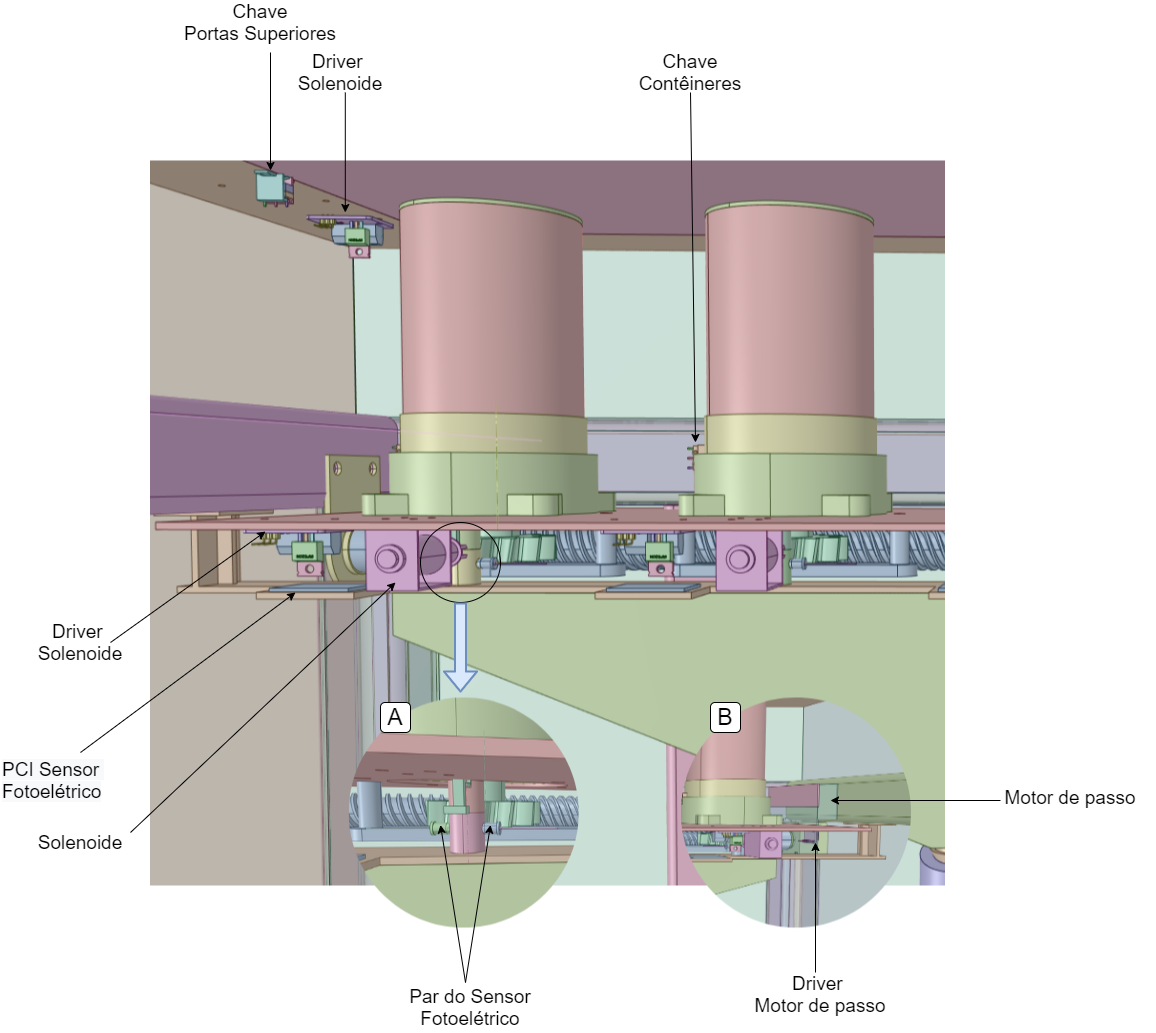
\includegraphics[width=\textwidth]{figuras/integracao/integracao_4.png} 
        \caption{}
        \label{fig:integracao_4}
    \end{figure}
    
    
\section{Alimentação dos Componentes Eletrônicos}
\label{alimentacao_componentes}

A partir do levantamento de carga do sistema, foi dimensionado e projetado um circuito para alimentação de seus dispositivos elétricos e eletrônicos, este é composto por uma fonte de alimentação principal (fonte chaveada) e auxiliar (bateria). As duas fontes possuem um sistema de operação em paralelo e saída de alimentação em 12 V. A tensão de operação das solenoides, motor da esteira, motores de passo, atuador linear e travas elétricas, assim como seus respectivos \textit{drivers}, é 12 V, portanto, podem ser diretamente alimentados através do circuito projetado, porém, os componentes eletrônicos necessitam de uma tensão de 5 a 3,3 V, o que impossibilita a conexão direta com o sistema projetado. Para resolver este problema, foi adicionado um conversor abaixador de tensão, em que converte a tensão de 12 V para 5 V. Este componente está ligado diretamente ao sensor de biometria, o visor e à \textit{Raspberry Pi}, este é responsável por alimentar com tensão de 5 V os quatro microcontroladores e o sensor de leitura RFID, e com 3,3 V câmera, sensor de temperatura e de umidade. O conversor abaixador foi definido após avaliar todas as cargas que seriam a ele conectadas, diretamente ou indiretamente. 
\hspace{2cm}    
\begin{figure}[H]
        \centering
        \hspace{-2cm}
        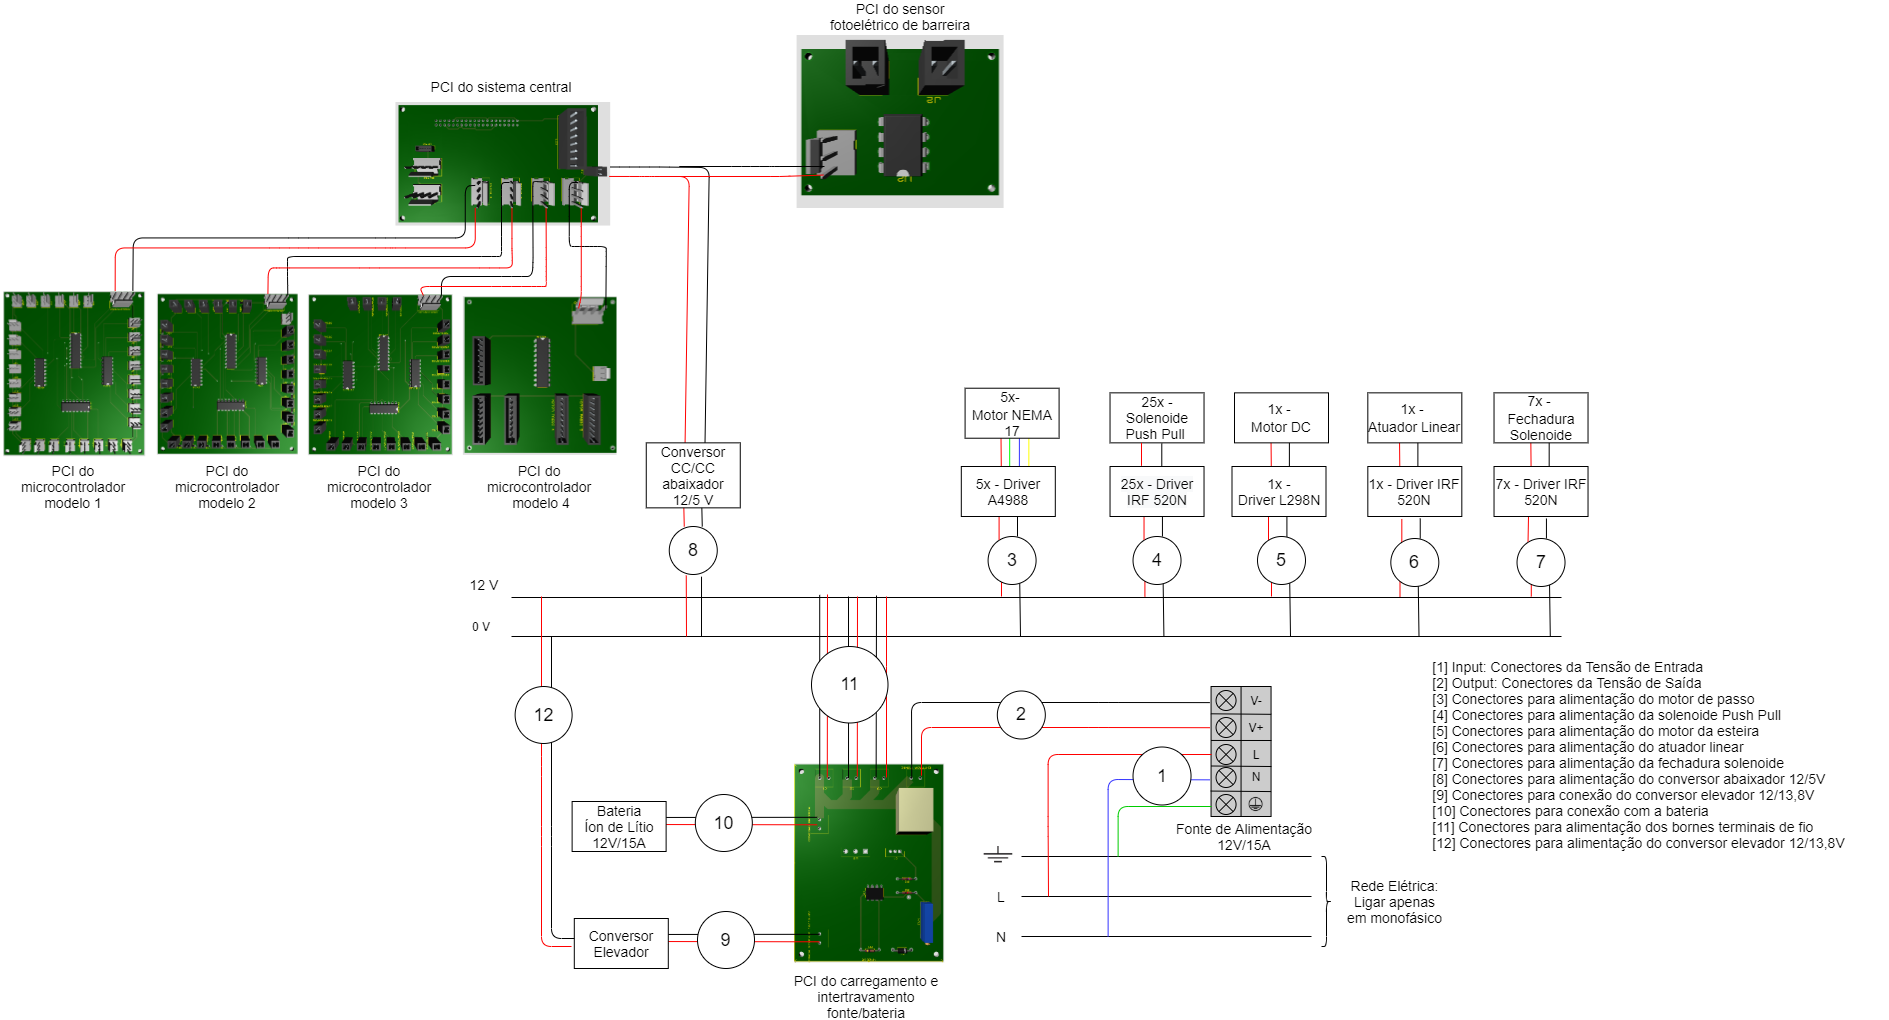
\includegraphics[width=1.1\textwidth]{figuras/integracao/integracao_energia_eletronica.png} 
        \caption{Diagrama de Alimentação dos componentes e Circuitos eletrônicos}
        \label{fig:integracao_eletrônica_energia}
    \end{figure}
    
    
\section{Comunicação entre o Aplicativo e o Dispositivo}
\label{app_dispositivo}

A comunicação entre o aplicativo e o dispositivo se dará por meio dos protocolos HTTP e MQTT, como já dito anteriormente, onde o sistema embarcado na central de controle se comunicará com o \textit{Back-end} da solução de Software.

Para a a comunicação MQTT, foram criados sete tópicos no \textit{Broker Mosquitto}, como descritos abaixo:

\begin{enumerate}
    \item \textbf{\textit{apply-medication}}: responsável por compartilhar mensagens contendo informações sobre a \textbf{medicação} a um paciente. Quando der o horário de alguma medicação a um determinado paciente, o \textit{back-end} enviará uma mensagem ao tópico, no formato do exemplo abaixo, para que o dispositivo leia essa mensagem e disponibilize a medicação.
    
    \begin{minted}[frame=single,
               framesep=3mm,
               linenos=true,
               xleftmargin=21pt,
               tabsize=4]{js}
    {
        "medicationId": 12,
        "nurseId": 5,
        "location": 25,
        "intervalTime": 8
    }
    \end{minted}
    
    \item \textbf{medication-response}: Após disponibilizar a medicação, o dispositivo envia uma mensagem ao \textit{back-end} confirmando o recebimento e processamento da requisição, seguindo o formato de mensagem:
    
    \begin{minted}[frame=single,
               framesep=3mm,
               linenos=true,
               xleftmargin=21pt,
               tabsize=4]{js}
    {
        "medicationId": 12,
        "nurseId": 5,
        "cupId": 1,
    }
    \end{minted}
    
    \item \textbf{create-nurse}: compartilha mensagens contendo informações de um \textbf{enfermeiro} recém criado. Sempre que um novo enfermeiro é cadastrado, o \textit{back-end} envia os dados do mesmo ao dispositivo. A mensagem segue o formato abaixo:
    
    \begin{minted}[frame=single,
               framesep=3mm,
               linenos=true,
               xleftmargin=21pt,
               tabsize=4]{js}
    {
        "coren": "123456",
        "document": "12345678910",
        "email": "logan.warden@email.com",
        "federativeUnit": "DF",
        "id": 1245,
        "imageUrl": "https://s3.com/image_from_user.jpg",
        "inclusionDate": "2020-01-21T17:32:28Z",
        "name": "Logan Warden",
        "phone": "992568745"
    }
    \end{minted}
    
    \item \textbf{create-patient}: compartilha mensagens contendo informações de um \textbf{paciente} recém criado. Sempre que um novo paciente é cadastrado, o \textit{back-end} envia os dados do mesmo ao dispositivo. A mensagem segue o formato abaixo:
    
        \begin{minted}[frame=single,
               framesep=3mm,
               linenos=true,
               xleftmargin=21pt,
               tabsize=4]{js}
    {
        "bornDate": "2020-11-08T18:34:44.347Z",
        "document": "71005638012",
        "id": 12345,
        "imageUrl": "https://s3.com/image_from_user.jpg",
        "inclusionDate": "2020-01-21T23:59:39Z",
        "name": "Logan Warden",
        "observation": "O paciente possui pressão alta;",
        "updateDate": "2020-01-21T23:59:39Z"
    }
    \end{minted}
    
    \item \textbf{create-prescription}: compartilha mensagens contendo informações de uma \textbf{receita} recém adicionada. Sempre que uma nova receita é adicionada a um paciente, o \textit{back-end} envia os dados do mesmo ao dispositivo. A mensagem segue o formato abaixo:
    
        \begin{minted}[frame=single,
               framesep=3mm,
               linenos=true,
               xleftmargin=21pt,
               tabsize=4]{js}
    {
        "id": 2,
        "imageUrl": "https://s3-amazon.com.br/daskjd",
        "inclusionDate": "2020-01-21T23:23:23Z",
        "patientCpf": "05389654102",
        "updateDate": "2020-11-08T18:41:24.433Z",
        "validityDate": "2020-11-08T18:41:24.433Z"
    }
    \end{minted}
    
    \item \textbf{create-medication}: compartilha mensagens contendo informações de uma \textbf{medicação} recém adicionada. Sempre que uma nova medicação é adicionada a uma receita de um paciente, o \textit{back-end} envia os dados da mesma ao dispositivo. A mensagem segue o formato abaixo:
    
        \begin{minted}[frame=single,
               framesep=3mm,
               linenos=true,
               xleftmargin=21pt,
               tabsize=4]{js}
    {
        "availableQuantity": 25,
        "batch": "0065560654545451294",
        "cupTag": "456055486512SDA",
        "expirationDate": "2020-11-08T18:38:11.159Z",
        "id": 2,
        "inclusionDate": "2020-01-21T23:23:23Z",
        "interval": 8,
        "location": 12,
        "medicine": {
            "dosage": 5,
            "dosageType": "MG",
            "id": 2,
            "inclusionDate": "2020-01-21T23:23:23Z",
            "name": "Novalgina"
        },
        "observation": "Tomar em jejum",
        "prescriptionId": 89,
        "quantity": 2,
        "startDate": "2020-11-08T18:38:11.160Z",
        "updateDate": "2020-11-08T18:38:11.160Z"
    }
    \end{minted}

    \item \textbf{create-supply}: Compartilha mensagens contendo informações de uma \textbf{solicitação de abastecimento}. Quando um enfermeiro precisa abastecer o dispositivo, ele faz a solicitação pelo aplicativo, esse se comunica com o \textit{back-end}, que envia uma mensagem ao tópico contendo as informações do abastecimento:
    
        \begin{minted}[frame=single,
               framesep=3mm,
               linenos=true,
               xleftmargin=21pt,
               tabsize=4]{js}
    {
        "id": 1,
        "inclusionDate": "2020-01-21T23:23:23Z",
        "medicationId": 76,
        "nurseId": 25,
        "quantity": 3
    }
    \end{minted}
\end{enumerate}

Para a comunicação HTTP, foi disponibilizada uma \href{http://192.99.25.198:8082/swagger-ui.html#/Patient/getPatientDetails}{URL} no \textit{back-end} para o dispositivo consultar informações completas sobre um paciente. Para essa consulta, o dispositivo precisa passar o identificador do paciente e terá como resposta a seguinte mensagem:

        \begin{minted}[frame=single,
               framesep=3mm,
               linenos=true,
               xleftmargin=21pt,
               tabsize=4]{js}
    {
        "id": 12345,
        "name": "Logan Warden",
        "prescription": [
            {
            "medication": [
                {
                "availableQuantity": 30,
                "cupTag": "456055486512SDA",
                "dosage": 25,
                "dosageType": "mL",
                "intervalTime": 30,
                "location": 17,
                "medicationId": 12345,
                "name": "Parecetamol"
                }
            ],
            "prescriptionId": 12345,
            "validityDate": "2020-11-08T18:48:59.191Z"
            }
        ]
    }
    \end{minted}